\section{Adafruit và thiết bị}
\subsection{Adafruit}
\subsubsection{Adafruit IO}
\indent Adafruit IO là một nền tảng IoTs (Internet of Things) dựa trên đám mây, giúp bạn thu thập, hiển thị và điều khiển dữ liệu từ các thiết bị kết nối internet. Đây là một dịch vụ miễn phí của Adafruit, hỗ trợ các giao thức REST API và MQTT, giúp dễ dàng kết nối các vi điều khiển như ESP8266, ESP32, Raspberry Pi, Arduino, STM32,...
\subsubsection{Các chức năng chính của Adafruit IO}
\begin{itemize}[leftmargin = 1cm]
	\item \textit{Feeds (Luồng dữ liệu):} Lưu trữ và quản lý dữ liệu từ cảm biến hoặc thiết bị.
	\item \textit{Dashboards (Bảng điều khiển):} Cung cấp giao diện đồ họa trực quan (biểu đồ, công tắc, nút bấm,...) để giám sát dữ liệu. Có thể tạo dashboard để điều khiển thiết bị từ xa.
	\item \textit{Giao thức MQTT:} Gửi dữ liệu theo thời gian thực, phù hợp với thiết bị IoT.
	\item \textit{Hỗ trợ nhiều nền tảng:} Có thư viện Adafruit IO Arduino và Adafruit MQTT giúp lập trình dễ dàng. Tích hợp với ESP8266, ESP32, Arduino, Raspberry Pi, STM32, Python,...
\end{itemize}
\subsubsection{Cách hoạt động của Adafruit IO}
\begin{itemize}[leftmargin = 1cm]
	\item Thiết bị IoT (ESP8266, ESP32,...) gửi dữ liệu lên Adafruit IO qua MQTT hoặc REST API.
	\item Adafruit IO lưu trữ và hiển thị dữ liệu trên giao diện trên feed.
	\item Người dùng có thể điều khiển thiết bị từ xa qua dashboard hoặc API. Tức là điều khiển thiết bị IoT bằng cách ra lệnh cho Adafruit IO thông qua Adafruit dashboard.
\end{itemize}

\subsection{Thiết kế hệ thống và lựa chọn thiết bị}
\indent Ở giai đoạn đầu, nhóm tiến hành phân tích yêu cầu của hệ thống nông nghiệp thông minh và lựa chọn các thiết bị phù hợp. Hệ thống được thiết kế gồm các thành phần chính:
\begin{itemize}[leftmargin = 1cm]
	\item \textbf{Cảm biến DHT20:} dùng để đo nhiệt độ và độ ẩm không khí.
	Cảm biến này cung cấp dữ liệu môi trường nền để hệ thống đánh giá điều kiện phát triển của cây và cập nhật lên dashboard.
	\begin{figure}[H]
		\centering
		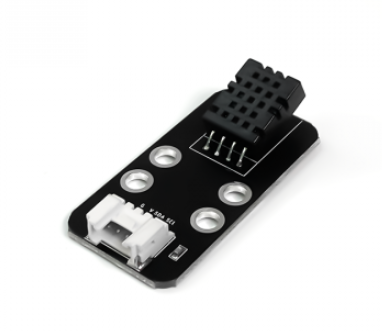
\includegraphics[width=0.45\linewidth]{./Pictures/Task_4/1_dht20.png}
		\caption{Cảm biến DHT20}
	\end{figure}
	\item \textbf{Cảm biến độ ẩm đất:} dùng để xác định tình trạng đất nhằm hỗ trợ hệ thống tưới tự động.
	Cảm biến giúp nhận biết đất đang khô hay đủ ẩm, từ đó làm căn cứ kích hoạt tưới nước hợp lý.
	\begin{figure}[H]
		\centering
		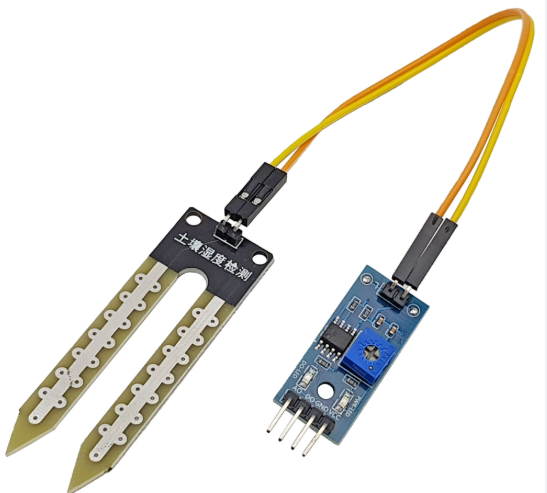
\includegraphics[width=0.45\linewidth]{./Pictures/Task_4/2_cb_doAmDat.png}
		\caption{Cảm biến độ ẩm đất}
	\end{figure}
	\item \textbf{Cảm biến ánh sáng:} để theo dõi cường độ ánh sáng trong môi trường.
	Dữ liệu từ cảm biến được dùng để kiểm tra mức chiếu sáng tại khu vực trồng và hỗ trợ đánh giá nhu cầu bổ sung ánh sáng.
	\begin{figure}[H]
		\centering
		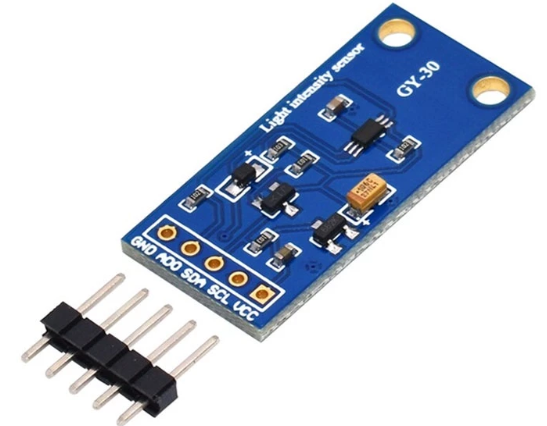
\includegraphics[width=0.45\linewidth]{./Pictures/Task_4/3_cb_anhSang.png}
		\caption{Cảm biến ánh sáng}
	\end{figure}
	\item \textbf{Đèn RGB:} dùng làm đèn báo trạng thái của hệ thống.
	Đèn RGB được dùng để hiển thị trạng thái hoạt động bằng màu sắc, giúp người dùng quan sát nhanh tình trạng hệ thống ngay tại thiết bị.
	\begin{figure}[H]
		\centering
		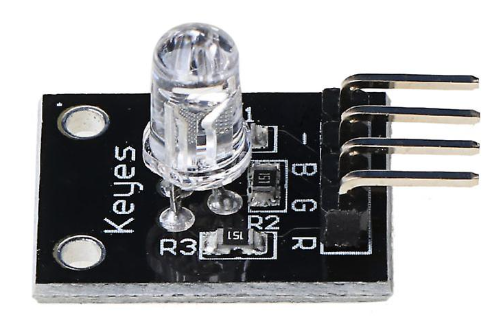
\includegraphics[width=0.45\linewidth]{./Pictures/Task_4/4_denRGB.png}
		\caption{Đèn RGB}
	\end{figure}
	\item \textbf{Màn hình LCD 16$\times$2:} để hiển thị các thông số môi trường trực tiếp tại thiết bị.
	Màn hình này cho phép quan sát trực tiếp các giá trị đo được mà không cần truy cập vào giao diện web.
	\begin{figure}[H]
		\centering
		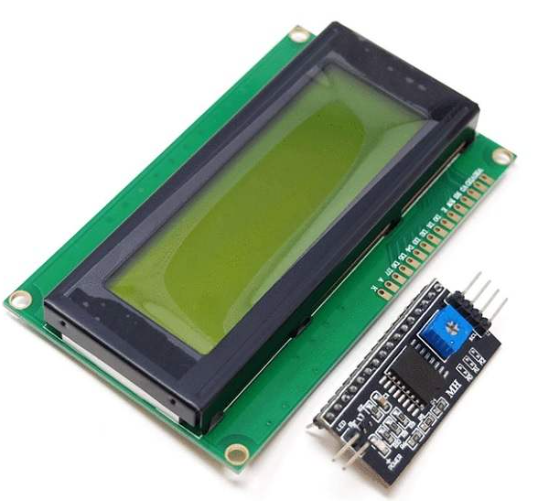
\includegraphics[width=0.45\linewidth]{./Pictures/Task_4/5_manHinhLCD.png}
		\caption{Màn hình LCD 16$\times$2}
	\end{figure}
	\item \textbf{Hai máy bơm nước:} phục vụ chức năng tưới tự động và tưới theo thời gian.
	Hai máy bơm đóng vai trò chấp hành, đưa nước đến cây trồng khi hệ thống cần tưới hoặc theo lịch đã thiết lập.
	\begin{figure}[H]
		\centering
		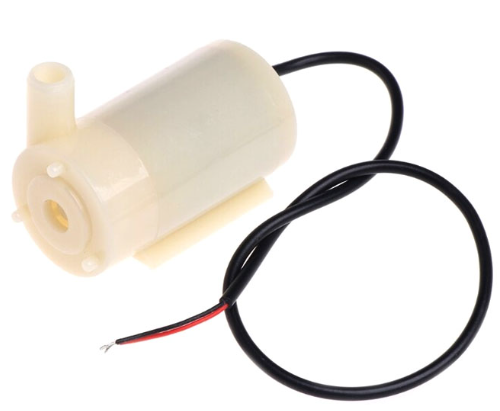
\includegraphics[width=0.45\linewidth]{./Pictures/Task_4/6_mayBom.png}
		\caption{Máy bơm mini}
	\end{figure}
\end{itemize}

\subsection{Kết nối phần cứng}
\indent Sau khi lựa chọn thiết bị, nhóm tiến hành thiết kế sơ đồ kết nối phần cứng. Trong hệ thống này, Yolo:Bit đóng vai trò là bộ điều khiển trung tâm, nhận dữ liệu từ các cảm biến, xử lý logic điều khiển và xuất tín hiệu đến các cơ cấu chấp hành, đồng thời là cầu nối giữa lớp phần cứng và lớp IoT.
\begin{figure}[H]
	\centering
	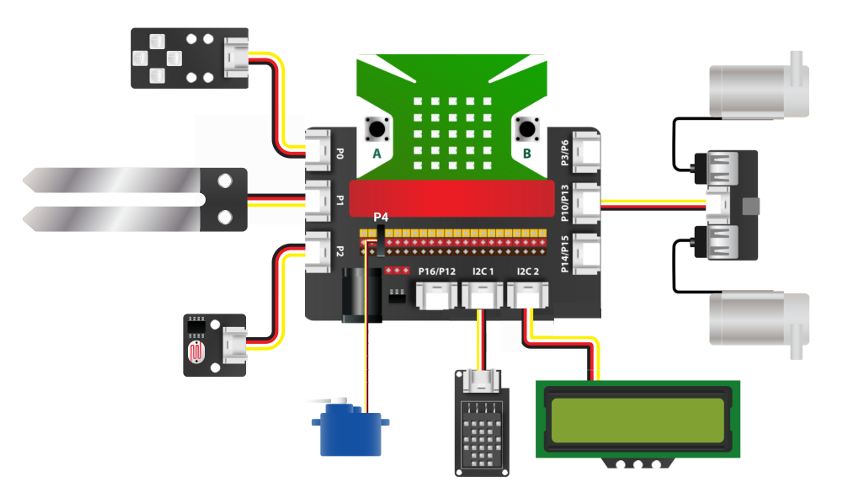
\includegraphics[width=1\linewidth]{./Pictures/Task_4/8_YoloBit_circuit.png}
	\caption{Kết nối thêm ngoại vi cho Yolo:Bit}
\end{figure}

\begin{itemize}[leftmargin = 1cm]
	\item \textbf{DHT20} được kết nối qua \textbf{I2C1} để đọc nhiệt độ và độ ẩm, là đầu vào chính cho việc giám sát môi trường.
	\item \textbf{LCD 16x2} sử dụng \textbf{I2C2} để hiển thị dữ liệu, giúp người dùng theo dõi thông số ngay tại thiết bị.
	\item \textbf{Cảm biến độ ẩm đất} được kết nối tại \textbf{P1} để đo tình trạng ẩm của đất phục vụ tưới tự động.
	\item \textbf{Cảm biến ánh sáng} được kết nối tại \textbf{P2} để ghi nhận cường độ chiếu sáng môi trường.
	\item \textbf{Đèn RGB} được kết nối tại \textbf{P0} để báo trạng thái hoạt động của hệ thống.
	\item \textbf{Động cơ RC} được điều khiển thông qua \textbf{P4} như một cơ cấu chấp hành trong quá trình vận hành.
	\item \textbf{Hai máy bơm} được điều khiển qua \textbf{P10} và \textbf{P13} để thực hiện chức năng tưới nước.
\end{itemize}
\indent Sau khi hoàn thành kết nối, hệ thống phần cứng đã hoạt động ổn định và có thể đọc dữ liệu từ các cảm biến.
\subsection{Thiết kế dashboard giám sát}
\begin{figure}[H]
	\centering
	
\includegraphics[width=1\linewidth]{./Pictures/Task_4/9_dashboard.png}
	\caption{Adafruit dashboard giám sát hệ thống}
\end{figure}
\indent Sau khi hoàn thành giao tiếp với server, nhóm tiến hành thiết kế Dashboard trên Adafruit IO để giám sát và điều khiển hệ thống từ xa.\\
\indent Dashboard bao gồm các \textit{gauges} để hiển thị giá trị tức thời, các \textit{cards} cho thông số quan trọng, các \textit{charts} để theo dõi lịch sử dữ liệu và các \textit{buttons} để điều khiển LED, máy bơm từ xa.
\begin{enumerate}[label = \arabic*., leftmargin = 1.7cm]
	\item Đồng hồ hiển thị nhiệt độ và độ ẩm.
	\item Đồng hồ hiển thị độ ẩm đất và cường độ ánh sáng.
	\item Các biểu đồ lịch sử dữ liệu cho nhiệt độ, độ ẩm và ánh sáng.
	\item Nút điều khiển LED và máy bơm từ xa.
\end{enumerate}
$\Longrightarrow$ Giao diện này cho phép người dùng theo dõi trạng thái môi trường và điều khiển thiết bị theo thời gian thực.